Алгоритм классификации Random Forest Classifier строится на двух базовых принципах: 
\begin{itemize}
  \item bagging --- мета-алгоритм в машинном обучении, при котором на основе большого числа <<слабых>> классификаторов (в данном случае деревьев решений) строится один <<сильный>> классификатор (рис.~\ref{forest:forest});
  \item метод случайных подпространств.
\end{itemize}

Преимущества данного алгоритма классификации:
\begin{itemize}
  \item способность эффективно обрабатывать данные с большим числом признаков и классов;
  \item нечувствительность к масштабированию (к любым монотонным преобразованиям) значений признаков;
  \item существует методы оценивания значимости отдельных признаков в модели;
  \item внутренняя оценка способности модели к обобщению (тест out-of-bag);
  \item высокая параллелизуемость и масштабируемость.
\end{itemize}

Недостатки алгоритма Random Forest Classifier:
\begin{itemize}
  \item алгоритм склонен к переобучению на некоторых задачах, особенно на зашумленных, однако для избежания переобучения используется энтропия Шеннона или коэффициент прироста информации (англ. Gain);
  \item большой размер получаемых моделей приводит к существенным затратам памяти на хранение деревьев, однако данный недостаток решается повышением вычислительных мощностей и распараллеливанием вычислений.~\cite{random_forest}
\end{itemize}

\begin{figure}[h!]
\center{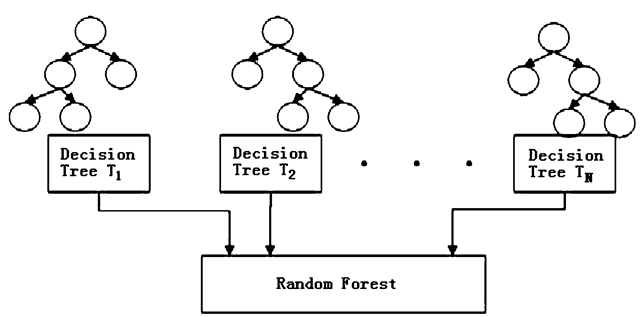
\includegraphics[width=0.7\linewidth]{forest}}
\caption{ Random Forest Classifier }
\label{forest:forest}
\end{figure} 
